\chapter{PDE Approach To Solving the Makean-Vlasov Equation}
\textcolor{Red}{This entire chapter needs alot of reworking, formulating Theorems etc. so there is more structure}
\section{Motivation}
Above we saw an SDE approach to solving the Makean-Vlasov Equation, in this section we instead focus on a PDE based approach.
From now on we assume $\sigma(Y(t),\mu(t)) = \sqrt{2} $ is a constant, then the \hyperref[MVE]{(MVE)} can be rewritten as
 \begin{align*}
   \text{(MVE*)}\begin{cases}
    Y(t) &= b(Y(t),\mu(t)) dt + \sqrt{2} dW_t\\
    Y(0) &= \xi \in  L^{2}(\Omega ) \\
    \mu_0 &= \mathcal{L}(\xi)
   \end{cases}
 .\end{align*}
 by applying It\^os formula for $\forall \phi  \in  \mathcal{C}_0^{\infty}([0,T)\times \mathbb{R}^{d} ) $
\begin{align*}
  \phi(Y(t),t) - \phi(Y(0),0) &= \int_0^{t} \frac{\partial \phi }{\partial t}(Y(s),s) + \nabla \phi(Y(s),s)*b(Y(s),\mu(s))  \\
                              &+ \frac{1}{2} \underbrace{\sqrt{2}*\sqrt{2})}_{tr(\sigma *\sigma ^{T} )}* \Delta \phi(Y(s),s) ds \\
                              &+ \int_0^{t} \nabla \phi(Y(s),s)  \sqrt{2} dW_s 
.\end{align*}
and taking the expectation  on both sides, such that the last term disappears 
\begin{align*}
  &\int_{\mathbb{R}^{d} } \phi(x,t) d\mu(t) - \int_{\mathbb{R}^{d} } \phi(x,0) d\mu_0 \\
  &= \int_0^{t} \int_{\mathbb{R}^{d} } \frac{\partial \phi }{\partial t}(x,s) + \nabla \phi(x,s)*b(x,\mu(s))* \Delta \phi(x,s)  d\mu(s) ds
.\end{align*}
This leads us to formulating the following weak PDE, if $\mu$ is regular enough i.e it has density and the density has enough regularity, then $\mu $ should satisfy 
\begin{align*}
  \begin{cases}
    &\partial_t \mu  - \Delta \mu  + \nabla * (b(x,\mu) * \mu )  =0\\
    &\mu(0) = \mu_0
  \end{cases}
.\end{align*}
\begin{remark}
 Compare this weak PDE to the one we got in the discrete case, what do you\\ notice ?
\end{remark}
\begin{exercise}
 Show that the integral equation and the weak formulation are equal.
\end{exercise}
\begin{remark}
 Now suppose we find $\mu $ with density $u$ satisfying the weak PDE, then we can plug it in to the \hyperref[MVE]{(MVE)} equation
 to get
 \begin{align*}
   \begin{cases}
    &dY_t = b(Y_t,u) dt + \sqrt{2} dW_t \\
    &Y(t) = \xi \in  L^2(\Omega ) \quad \mathcal{L}(\xi) = u
  \end{cases}
 .\end{align*}
 Now if $b$ is bounded and Lipschitz continuous, then we get a solution $Y_t $. Now if $\overline{u} $ is the Law of $Y_t$.
 Then by It\^o formula we have for $\forall  \phi \in \mathcal{C}_0^{\infty} $
\begin{align*}
  &\int_{\mathbb{R}^{d} } \phi (x,t) d\overline{\mu(t)}  - \int_{\mathbb{R}^{d} } \phi(x,0) u_0(x) dx \\
  &=  \int_0^{t} \int_{\mathbb{R}^{d} } \left(\frac{\partial \phi }{\partial t}(x,s) + \nabla \phi(x,s)*b(x,u) -  \Delta \phi(x,s)\right)\overline{u}(x,t) dx ds
.\end{align*}
Which means $\overline{\mu } $ satisfies
\begin{align*}
  \begin{cases}
    &\partial_t \overline{\mu }  - \Delta \overline{\mu }  + \nabla * (b(x,u)*\overline{\mu } ) = 0\\
    &\overline{\mu } \rvert_{t=0}  = u_0
  \end{cases}
.\end{align*}
If we can prove $\overline{u} = u $, then we get a solution to the \nameref{MVE}. 
\end{remark}
\begin{example}
 A common choice of $b$ is the following for some kernel $K$
\begin{align*}
  b(Y_t,u) = \int K(Y_t-y)u(y) dy = \int K(y)u(Y_t-y) dy
.\end{align*}
then the regularity of $b$ by convolution depends on either $K$ or $u$
\end{example}
\section{Problem Definition}
\begin{definition}[Weak PDE]\label{weak_pde_mve}
  Let $\mu $ have density $u$, then we write 
  \begin{align*}
    \text{(PDE)}\begin{cases}
    &\partial_t u  - \Delta u  + \nabla * (b(x,u)*u )  =0\\
    &u(0) = u_0
  \end{cases}
.\end{align*}
\todo{Formalize by adding the relevant spaces}
\end{definition}
\begin{definition}[Sobolev Spaces]
 We define roughly  
 \begin{align*}
   H^1(\mathbb{R}^{d} ) &= \{u \in  L^2(\mathbb{R}^{d})  :  \nabla u \in  L^2(\mathbb{R}^{d}) \}  \\
   \|u\|_{H_{1}} &= \|u\|_2 + \|\nabla u\|_2
 .\end{align*}
 where the gradient is defined for $\forall  \phi \in  \mathcal{C}_0^{\infty} $ 
 \begin{align*}
   \nabla u = \braket{\nabla u , \phi } = -\braket{u,\nabla \phi }
 .\end{align*}
 And the dual space
 \begin{align*}
  H^{-1}(\mathbb{R}^{d} )  =  (H^{1}(\mathbb{R}^{} ) )' =  \{l : l\text{ is bounded linear functional of } H^{1}(\mathbb{R}^{d} )  \}  
 .\end{align*}
 Then  
 \begin{align*}
   L^2([0,T];H^{1}(\mathbb{R}^{d} ) ) = \{u : \int_0^{T} \|u(t)\|_{H^1} dt < \infty \}  
 .\end{align*}
\end{definition}
\begin{remark}
 The Sobolev space $H^1$ is a separable Hilbert space 
\end{remark}
\begin{definition}[Weak Solution]
  We say that a function 
  \begin{align*}
    u \in  L^2([0,T];H^{1}(\mathbb{R}^{d} )\cap L^{\infty}([0,T];L^2(\mathbb{R}^{d} ))  )
  .\end{align*}
  with $\partial_t u \in  L^2([0,T];H^{-1}(\mathbb{R}^{d} ))$ is a weak solution of the \hyperref[weak_pde_mve]{(PDE)} if for
  $\forall  \phi  \in \mathcal{C}^{\infty}_0([0,T]\times \mathbb{R}^{d} )  $ it holds 
  \begin{align*}
    \int_0^{T} \braket{\partial_t u , \phi }_{(H^{-1},H^{1})} dt &= \int_0^{T} \int_{\mathbb{R}^{d} }  \nabla \phi * (b(x,u)*u) dx dt \\
                                                                 &- \int_0^{T} \int_{\mathbb{R}^{d} }  \nabla u * \nabla \phi  dx dt
  .\end{align*} 
\end{definition}
\section{Heat Equation and the Heat Kernel}
\subsection{Motivation}
\begin{definition}[Heat equation]\label{HE}
 The following PDE is called the inhomogenes Heat equation with source term $f$ 
 \begin{align*}
   \text{(HE)}\begin{cases}
   \partial_t u(x,t) - \Delta u(x,t) &=f(x,t)\\
   u \rvert_{t=0} &= u_0
 \end{cases} 
 .\end{align*}
\end{definition}
\begin{remark}
 Compare this to our PDE which looks similar, but is in fact non-linear 
\begin{align*}
 \partial_t u - \Delta u + \nabla * (b(x,u)*u) = 0
 .\end{align*}
\end{remark}
\begin{remark}
 Let us suppose $K(x,t)$  is a heat kernel, then 
  \begin{align*}
    u(x,t) &=  \int_{\mathbb{R}^{d} } K(x-y,t) u_0(y) dy - \int_0^{t} \int_{\mathbb{R}^{d} }  K(x-y,t-s) \nabla * (b(y,u(y,s)u(y,s))dy ds \\
           &= u_{1}(x,t) + u_{2}(x,t)
  .\end{align*}
  is a solution to the inhomogenous Heat-Equation, this is called Duhamel's principle i.e. we can "add" up solutions
  to homogeneous problems and get the solution to the inhomogenous.
\end{remark}
\begin{remark}
 We say the heat kernel is the density of the Brownian Motion. 
\end{remark}
\subsection{Derivation by Fourier Transform}
\begin{definition}[Fourier Transform]
 For $x \in  \mathbb{R}^{d} $ the Fourier transform is defined as
\begin{align*}
  \mathcal{F} : L^2 \to  L^2 \ u \mapsto \hat{u} 
.\end{align*}
where
\begin{align*}
  \hat{u} (k) = \int_{\mathbb{R}^{d} } u(x) e^{ix*k}  dx 
.\end{align*}
\end{definition}
\begin{exercise}
  Proof
\begin{align*}
  - \widehat{\Delta u}  = \abs{k}^2 \hat{u}(k)
.\end{align*}
\textit{Hint} 
\begin{align*}
  \widehat{\nabla u} = \frac{k}{i} \hat{u}(k)
.\end{align*}
\end{exercise}
\begin{remark}
 Using the Fourier transformation we can transform our PDE into an ODE 
\begin{align*}
  \begin{cases}
    \partial_t \hat{u} - \widehat{\Delta u} &=\hat{f}\\
   \hat{u} \rvert_{t=0} &= \hat{u}_0
 \end{cases} 
 .\end{align*}
 that is
 \begin{align*}
   \begin{cases}
     &\partial_t \hat{u}(k)  + \abs{k}^2 \hat{u} (k) = \hat{f}(k) \\
     &\hat{u}_0(k)= \hat{u}_0
   \end{cases}
 .\end{align*}
 where 
\begin{align*}
  \hat{u} (k,t)= e^{-\abs{k}^2t} \hat{u}_0(k) + \int_0^{t}  e^{-\abs{k}^2(t-\tau )} \hat{f}(k,\tau ) d \tau 
 .\end{align*}
\end{remark}
\begin{lemma}[Inverse transformation of the Fourier transformation]
 \begin{align*}
   u(x,t) =  \frac{1}{(4\pi t)^{\frac{d}{2}} }\int_{\mathbb{R}^{d} } e^{-\frac{\abs{x-y}^2}{4t}} u_0(y) dy + \int_0^{t} \int_{\mathbb{R}^{d} }   \frac{1}{(4\pi(t-\tau ))^{\frac{d}{2}} } e^{\frac{-\abs{x-y}^2}{4(t-\tau )}} f(y,\tau )dy d\tau 
 .\end{align*}
\end{lemma}
\begin{definition}[Heat Kernel]
 The following is called Heat Kernel
 \begin{align*}
  K(x,t) = \frac{1}{(4\pi t)^{\frac{d}{2}} } e^{-\frac{\abs{x}^2}{4t}} 
 .\end{align*}
 and for $\forall  t > 0 $ it is a solution to the homogeneous heat equation
 \begin{align*}
  \partial_t K - \Delta K  = 0
 .\end{align*}
 And 
 \begin{align*}
   K \xrightarrow{t \to 0^{+} } \delta 
 .\end{align*}
 In the sense of distributions.
\end{definition}
\begin{theorem}[Solution To Heat Equation]
  Let $K$  be the Heat kernel and initial data $u_{0} \in \mathcal{C}_b(\mathbb{R}^{d} )$ and $f \in  \mathcal{C}^{2,1}(\mathbb{R}^{d} \times  [0,T]) $ with compact support (schwarz function would work as well, since they lie dense in compact)
\begin{align*}
    u(x,t) &=  \int_{\mathbb{R}^{d} } K(x-y,t) u_0(y) dy - \int_0^{t} \int_{\mathbb{R}^{d} }  K(x-y,t-s) \nabla * (b(y,u(y,s)u(y,s))dy ds \\
           &= u_{1}(x,t) + u_{2}(x,t)
  .\end{align*}
  is a solution to the heat equation, in fact $u_{1}$ and $u_{2}$ are solutions to
  \begin{align*}
    \text{(P1)}\begin{cases}
      &\partial_t u_{1} - \Delta u_{1} = 0 \\
      &u_{1}(0) = u_{0}
    \end{cases}
    \qquad 
    \text{(P2)}\begin{cases}
      &\partial_t u_{2} - \Delta u_{1} = f \\
      &u_{2}(0) = u_{0}
    \end{cases}
  .\end{align*}
  respectively
\end{theorem}
\begin{proof}
  We begin by showing that $u_{1}$ is a solution to (P1) by showing
  \begin{align*}
    \lim_{t \to 0^{+}}  u_{1}(x,t) = \lim_{t \to 0^{+}} \int_{\mathbb{R}^{d} }K(x-y,t)u_0(y) dy \myS{!}{=} u_{0}
  .\end{align*}
  \begin{align*}
    \lim_{t \to 0^{+} }\int_{\mathbb{R}^{d} }K(x-y,t)u_0(y) dy &= \lim_{t \to 0^{+} } \int_{\mathbb{R}^{d} } \frac{1}{(4\pi t)^{\frac{d}{2}}} e^{-\frac{\abs{x-y}^2}{4t}} u_0(y) dy \\ 
                                           &=  \lim_{t \to 0^{+} } \int_{\mathbb{R}^{d} } \frac{1}{(4\pi t)^{\frac{d}{2}} } e^{-\abs{z}^2}  u_{0}(x+2 \sqrt{t} z ) dz \\
                                           &= \int_{\mathbb{R}^{d}  } \lim_{t \to 0^{+} } \frac{1}{(4\pi t)^{\frac{d}{2}} } e^{-\abs{z}^2}  u_{0}(x+2 \sqrt{t} z ) dz \\
                                           &= u_0(x)  
  .\end{align*}
  where we used the change of variables 
  \begin{align*}
    \frac{x-y}{2 \sqrt{t} }= -z
  .\end{align*}
  Then  for $\forall  t > 0$
  \begin{align*}
    \partial_t u_{1} - \Delta u_{1} &= (\partial_t -  \Delta) \int_{\mathbb{R}^{d} } K(x-y,t)u_0(y)dy\\
                                    &= \int_{\mathbb{R}^{d} } (\partial_t - \Delta )K(x-y,t) u_0(y) dy \\
                                    &= 0
  .\end{align*}
  by properties of the Heat-Kernel. \\[1ex]
  For $u_{2}(x,t)$ , we further assume $f$ has compact support
  \begin{align*}
    u_{2}(x,t)  = \int_0^{t}  \int_{\mathbb{R}^{d} }K(y,s)f(x-y,t-s) dy ds
  .\end{align*}
  First note that  
  \begin{align*}
    \lim_{t \to 0^{+}}  u_{2}(x,t) &= 0 
  .\end{align*}
  Then by applying 
  \begin{align*}
    (\partial_t - \Delta )u_{2}  &= \int_0^{t} \int_{\mathbb{R}^{d} } K(y,s)(\partial_t - \Delta_x)f(x-y,t-s) dy ds \\
                                 &+ \int_{\mathbb{R}^{d} } K(y,t)f(x-y,0) dy\\
                                 &=  \int_{0}^{\epsilon} \int_{\mathbb{R}^{d} } K(y,s) \left( -\partial_s - \Delta_y \right)f(x-y,t-s) dy ds +  \int_{\epsilon}^{t} \int_{\mathbb{R}^{d} } \ldots  \\
                                 &+   \int_{\mathbb{R}^{d} } K(y,t)f(x-y,0) dy\\
                                 &= I_{\epsilon} +  J_{\epsilon} + L
  .\end{align*}
  We are allowed to exchange the order because of the Heat-Kernel since it decays very fast this gives uniform integrability the further away we get from the origin\\
  We have, since $f \in  \mathcal{C}_b^{2,1}  $ we get that its term is bounded and the integral for the Heat kernel is just 1
  \begin{align*}
    \abs{I_\epsilon} &\le  C*\epsilon\\
    J_{\epsilon} &= \int_{\epsilon}^{t}  \int_{\mathbb{R}^{d} } K(y,s)(-\partial_t - \Delta_y) f(x-y,t-s)dy ds\\
                 &= \int_{\epsilon}^{t}  \int_{\mathbb{R}^{d} } \underbrace{(-\partial_t - \Delta_y)K(y,s)}_{=0}f(x-y,t-s)dy ds\\ 
                 &+ \int_{\mathbb{R}^{d} }K(y,\epsilon) - f(x-y,t-\epsilon) dy \\
                 &-\underbrace{\int_{\mathbb{R}^{d} } K(y,t) f(x-y,0) dy}_{=Li }
  .\end{align*}
\end{proof}
Together we have 
\begin{align*}
  \partial_t u_{2} - \Delta u_{2} &= \lim_{\epsilon \to 0} \left( \int_{\mathbb{R}^{d} } \underbrace{K(y,\epsilon)}_{\to \delta} f(x-y,t-\epsilon) dy + \underbrace{C\epsilon}_{\to 0} \right)  \\
                                  &= f(x,t)
.\end{align*}
This shows that 
\begin{align*}
  u(x,t) &=  \int_{\mathbb{R}^{d} } K(x-y,t) u_0(y) dy - \int_0^{t} \int_{\mathbb{R}^{d} }  K(x-y,t-s) \nabla * (b(y,u(y,s)u(y,s))dy ds \\
.\end{align*}
is a solution to the inhomogenous heat equation. 
\begin{remark}
  When changing order or variable of derivative one has to be aware of the boundary terms appearing.
 For example when changing the order for the $\partial_t$  derivative one gets two boundary terms , where one is not well behaved $t=0$
\end{remark}
\begin{align*}
  \begin{cases}
    &\partial_t u  - \Delta u + \nabla * (b(x,u)*u) = 0\\
    &u \rvert_{t=0} =u_{0} \in  L^{1} \ \int (1+\abs{x}^2)u_{0} <\infty
  \end{cases}
.\end{align*}
Formally
\begin{align*}
  u(x,t)  = \int_{\mathbb{R}^{d} } K(x-y,t)u_{0}(y) dy - \int_0^{t} \int_{\mathbb{R}^{d} }K(x-y,t-\tau ) \nabla * (b(y,u(y,\tau ))*u(y,\tau ))dy d\tau 
.\end{align*}
Now we start with bounded drift term for a linear equation.
\begin{definition}[LDE]\label{LDE}
  For bounded drift term $\overline{b} \in  L^{\infty}  $ we define
\begin{align*}
  \text{(LDE)}\begin{cases}
    &\partial_t - \Delta u + \nabla * (\overline{b}(x,t)u ) = 0 \\ 
    & u \rvert_{t=0} = u_{0}
  \end{cases}
.\end{align*}
\end{definition}
\begin{remark}
  By first proving the existence of a solution to this simpler equation we can then construct an iteration that will yield
a solution to the more complex non-linear , non-local one.
\end{remark}
\begin{theorem}[Uniqueness and Existence of LDE Solution ]
  If $b \in  L^{\infty}([0,T] \times  \mathbb{R}^{d} ) $  and $u_{0} \in  L^1(\mathbb{R}^{d} )$, then the \hyperref[LDE]{(LDE)} has a 
  unique solution $u \in L^{\infty}([0,T];L^{1}(\mathbb{R}^{d} ) ) $
  \begin{align*}
    u(x,t) = \int_{\mathbb{R}^{d} }K(x-y,t)u_{0}(y) dy  + \int_{0}^{t} \int_{\mathbb{R}^{d} } \nabla K(x-y,t-\tau ) * (\overline{b}(y,\tau )u(y,\tau ) ) dy d\tau 
  .\end{align*}
\end{theorem}
\begin{proof}
 We prove again by Iteration, and fix point argument, consider a map 
 \begin{align*}
   &\mathcal{T} : L^{\infty}([0,T];L^1(\mathbb{R}^{d} )) \to L^{\infty}([0,T];L^1(\mathbb{R}^{d} ))\\
   &u \mapsto \mathcal{T}(u) = \int_{\mathbb{R}^{d} }K(x-y,t)u_{0}(y) dy  + \int_{0}^{t} \int_{\mathbb{R}^{d} } \nabla K(x-y,t-\tau ) * (\overline{b}(y,\tau )u(y,\tau ) ) dy d\tau 
 .\end{align*}
 We need to check $\mathcal{T}(u) \in  L^{\infty}([0,T];L^{1}(\mathbb{R}^{d} ) ) $, for $\forall  t >0$
 \begin{align*}
   \int_{\mathbb{R}^{d} }\abs{\mathcal{T}(u)(x,t)} dx &\le \int_{\mathbb{R}^{d} } \int_{\mathbb{R}^{d} } K(x-y,t)\abs{u_0(y)}dy dx \\
                                                      &+ \int_0^{t}  d\tau \int_{\mathbb{R}^{d} }dx \int_{\mathbb{R}^{d} } dy \abs{\nabla K(x-y,t-\tau )\overline{b} (y,\tau )u(y,\tau )}\\
                                                      &= I + II
 .\end{align*}
  Since we have fixed $t >0$ we use Fubini 
  \begin{align*}
    I &\le \int_{\mathbb{R}^{d} }\underbrace{\int_{\mathbb{R}^{d} }K(x-y,t) dx}_{=1} \abs{u_0(y)}dy\\
      &\le \|u_{0}\|_{L^{1}(\mathbb{R}^{d} ) }
  .\end{align*}
  First consider the gradient of $K$
  \begin{align*}
    \int_{\mathbb{R}^{d} }\nabla K(x,s) dx  &= \frac{1}{(4 \pi s)^{\frac{d}{2}} } \int_{\mathbb{R}^{d} } \frac{1}{\sqrt{s} }\abs{\frac{4}{2 \sqrt{s} }} e^{-\frac{\abs{x}^2}{4s}} dx \\
                                            &\le  \frac{1}{\sqrt{s} }C
  .\end{align*}
  Then for the second term we get 
  \begin{align*}
    II &\le  \|\overline{b} \|_{L^{\infty} }\int_{0}^{t}  d\tau  \int_{\mathbb{R}^{d} } \abs{\nabla K(x,t-\tau )}dx \int_{\mathbb{R}^{d} }u(y,\tau )dy\\
       &\le \|\overline{b} \|_{L^{\infty} } \|u\|_{L^{\infty}(L^1) } C*\int_0^{t}  \frac{1}{\sqrt{s} } dy \\
       &=  C*\sqrt{t-\tau } 
  .\end{align*}
  Note we we do not need to consider $y$ in $K$ since we can use a translation,$L^{\infty}(L^{1} ) = L^{\infty}([0,T];L^{1}(\mathbb{R}^{d} ) )  $ \\[1ex]
  This shows that our map $\mathcal{T}$ is indeed well defined, next we proof $\mathcal{T}(u)$ is a contraction,
  for $\forall  u_{1},u_{2} \in  L^{\infty}(L^{1} ) $, for $t^{\star }$ s.t. $C \|\overline{b} \|_{\infty} \sqrt{t^{\star }} < \frac{1}{2} $
  \begin{align*}
    &\|\mathcal{T}(u_{1}) - \mathcal{T}(u_{2})\|_{L^{\infty}(L^{1} ) } \\
    &= \essup_{0\le t\le t^{\star} }\int_{\mathbb{R}^{d} } \abs{\mathcal{T}(u_{1}) - \mathcal{T}(u_{2})}(x,t)dx \\
    &\le  \essup_{0\le t\le t^{\star} } \int_0^{t} d\tau  \int_{\mathbb{R}^{d} } dy \abs{\nabla K(x-y,t-\tau )(\overline{b}(y,\tau )(u_{1}-u_{2}) )(y,\tau ) }\\
    &\le \essup_{0\le t\le t^{\star} } \|\overline{b} \|_{L^{\infty} }  \|u_{1}-u_{2}\|_{L^{\infty}(L^{1} ) } \int_0^{t} \frac{1}{\sqrt{t-\tau } } d \tau \\
    &\le \essup_{0\le t\le t^{\star} } C\|\overline{b} \|_{L^{\infty} } \sqrt{t}  \|u_{1}-u_{2}\|_{L^{\infty}(L^{1} ) }\\
    &\le C \|\overline{b} \|_{\infty} \sqrt{t^{\star }} \|u_{1}-u_{2}\|_{L^{\infty}(L^{1} ) }
  .\end{align*}
  Then  $\mathcal{T}$ is a contraction. Since $t^{\star }$ only depends on $\|\overline{b} \|_{\infty}$ and dimension d.
  Then for any given $T>0$ we can repeat the above argument finite many time and obtain
  \begin{align*}
    u \in  L^{\infty} ([0,T];L^{1}(\mathbb{R}^{d} ) )
  .\end{align*}
\end{proof}
\begin{exercise}
 Think about wether you can proof it for $b$   satisfying linear growth condition 
 \begin{align*}
  \abs{\overline{b} } \le  C(1+\abs{x})
 .\end{align*}
\end{exercise}
Let us discuss how a solution to the LDE leads back to a solution to the more complex 
\begin{align*}
  \partial_t u - \Delta u + \nabla * (b(x,u)u) = 0
.\end{align*}
where $u \in  L^{\infty}(L^{1} ) $ under the assumption on $b(x,u)$
\begin{align*}
  \abs{b(x,u) - b(\tilde{x},\tilde{u}  )} \le  L(\abs{x-\tilde{x} } + W_2(u,\tilde{u} ))
.\end{align*}
By fixing  $\tilde{x} = 0 $
\begin{align*}
  \abs{b(x,u) - b(0,\delta_0  )} \le  L(\abs{x} + W_2(u,\delta_0 )) \le L(1+\abs{x})
.\end{align*}
where 
\begin{align*}
  W_2(u,\delta_0) \le  \left(\int_{\mathbb{R}^{d} } \abs{x}^2 u(x) dx\right)^{\frac{1}{2}} 
.\end{align*}
when $b$ is unbounded we consider , the cutoff  
\begin{align*}
  \overline{b}(x,v(x,t))  = \min \{b(x,v(x,t)), M\}  
.\end{align*}
\begin{remark}
 In the (SDE)  case we would assume 
\begin{align*}
   \nabla V \in  \text{Lip} \tag{SDE}
 .\end{align*}
 since our (SDE) is given by
 \begin{align*}
  d X_i = \nabla V \star  u(x_i) dt + \sqrt{2} dW_t
 .\end{align*}
 and we know a solution to the linear SDE exists for Lipschitz continuous coefficients 
\end{remark}
\begin{definition}\label{pde_mve_apprach}
 Assume $b(x,u) $  is given by the convolution
 \begin{align*}
  b(x,u) = \nabla V \star u(x)
 .\end{align*}
 And let our (PDE) be given by 
 \begin{align*}
  \text{(PDE)}\begin{cases}
    &u_t - \Delta u + \nabla*(\nabla V \star  u \ u) = v\\
    &u \rvert_{t=0} = u_{0} \in  L^{1}((1+\abs{x}^2)dx) \cap L^{2}(dx) 
  \end{cases}
 .\end{align*}
\end{definition}
% \begin{definition}[Epsilon Problem]
%  We consider for $\epsilon > 0$  the problem
%  \begin{align*}
%    \text{(PDE)}_{\epsilon}\begin{cases}
%     &u_t^{\epsilon} - \Delta u^{\epsilon}  + \nabla*(j_{\epsilon}\star \nabla V \star  u^{\epsilon}  \cha_{\abs{x}\le \frac{1}{\epsilon}} \ u^{\epsilon} ) = v\\
%     &u^{\epsilon}  \rvert_{t=0} = \tilde{j}_{\epsilon} \star  u_{0} 
%   \end{cases}
%  .\end{align*}
% where  $j_{\epsilon}$ is the mollification kernel in $x,t$ 
% \begin{align*}
%   \nabla V \star  u &\leftarrow j_{\epsilon} \star  \nabla V \star  u\\
%   u &\leftarrow j_{\epsilon} \star (\cha_{\abs{x} \le  \frac{1}{\epsilon}u})\\
%   u_0 &\leftarrow \tilde{j}_{\epsilon}  \star  u_{0}
% .\end{align*}
% where $\tilde{j}_{\epsilon} $ is mollification just in $x$
% \end{definition}
\begin{definition}[Epsilon Problem]
  For $v \in  L^{\infty}(L^{1} )$ consider $j_{\epsilon} \star  \nabla  V \star  v \leftarrow \nabla V \star  v $
 \begin{align*}
   \text{(PDE)}_{\epsilon}\begin{cases}
    &u_t^{\epsilon} - \Delta u^{\epsilon}  + \nabla*(j_{\epsilon}\star \nabla V \star  v \ (j_{\epsilon} \star \cha_{\abs{x}\le \frac{1}{\epsilon}} \ u^{\epsilon} )) = v\\
    &u^{\epsilon}  \rvert_{t=0} = \tilde{j}_{\epsilon} \star  u_{0} 
  \end{cases}
 .\end{align*}
where  $j_{\epsilon}$ is the mollification kernel in $x,t$ 
\begin{align*}
  \nabla V \star  u &\leftarrow j_{\epsilon} \star  \nabla V \star  u\\
  u &\leftarrow j_{\epsilon} \star (\cha_{\abs{x} \le  \frac{1}{\epsilon}u})\\
  u_0 &\leftarrow \tilde{j}_{\epsilon}  \star  u_{0}
.\end{align*}
where $\tilde{j}_{\epsilon} $ is mollification just in $x$
\end{definition}
\begin{remark}
  We first solve this problem for $v$, and then construct a fixpoint argument to get a solution for $u$, in order to solve $\text{PDE}$ ,
  for bounded $\overline{b}$ we already have a solution  
  \begin{align*}
    v \in  L^{\infty}(L^{1} ) \xrightarrow{\text{sol for bounded } \overline{b} } u \in  L^{\infty}(L^{1} ) 
  .\end{align*}
  Where we know our solution is given by 
  \begin{align*}
    u(x,t) = \int_{\mathbb{R}^{d} } K(x-y,t)u_{0}(y) dy + \int_0^{t}  \int_{\mathbb{R}^{d} } K(x-y,t-s) \nabla*(\nabla V \star  v \ u)(s,y) dy ds
  .\end{align*}
  We further want that 
  \begin{align*}
    \lim_{\abs{x} \to  \infty}u(x,t) = 0
  .\end{align*}
\end{remark}
\begin{remark}
 For the linear PDE with  term  
 \begin{align*}
  j_{\epsilon}\star \nabla V \star  v \ (j_{\epsilon} \star \cha_{\abs{x}\le \frac{1}{\epsilon}} \ u^{\epsilon} )
 .\end{align*}
 We get 
 \begin{align*}
   u^{\epsilon}(x,t) = \int_{\mathbb{R}^{d} } K(x-y,t)j_{\epsilon} \star u_{0}(y) dy + \int_0^{t}  \int_{\mathbb{R}^{d} } K(x-y,t-s) \nabla*(j_{\epsilon} \star \nabla V \star  v \ j_{\epsilon} (\cha_{\abs{x} \le  \frac{1}{\epsilon})} u^{\epsilon} ))(s,y) dy ds
 .\end{align*}
 then $u^{\epsilon} $ satisfies the eq. In the classical sense 
 \begin{align*}
  \begin{cases}
    &\partial_t u^{\epsilon}  - \Delta u^{\epsilon}  + \underbrace{\nabla*(j_{\epsilon}\star \nabla V \star  v \ (j_{\epsilon} \star \cha_{\abs{x}\le \frac{1}{\epsilon}} \ u^{\epsilon} ))}_{\in \mathcal{C}_0^{2,1} } = 0 \\ 
    &u^{\epsilon}  \rvert_{t=0} = \tilde{j}_{\epsilon} \star  u_{0}
  \end{cases}
 .\end{align*}
\end{remark}
\begin{lemma}[Estimates]
   We have $u \in  L^{\infty}(L^{1} ) =  L^{\infty}([0,T];L^{1}(\mathbb{R}^{d} ) ) $ 
\end{lemma}
   \begin{proof}
    
     \begin{align*}
       \|u^{\epsilon} \|_{L^{\infty}(L^{1} ) } &= \sup_{t} \int_{\mathbb{R}^{d} }\abs*{I(x,t) + II(x,t)}dx\\
                                               &\le \sup_t \int_{\mathbb{R}^{d} } \abs*{\int_{\mathbb{R}^{d} } K(x-y,t)j_{\epsilon} \star u_{0}(y)} dy dx + II\\
                                               &\le \|K(t,*)\|_{L^{1} } * \|j_{\epsilon} \star  u_0\|_{L^{1} } + \|II\|\\
                                               &\le \|u_0\|_{L^{1} } + \|II\| \\
                                               &\le C_0 + C \sqrt{t}  \|u^{\epsilon} \|_{L^{\infty}(L^{1} ) }
     .\end{align*}
 Then for $C \sqrt{t^{\star }} \le \frac{1}{2}$ we have $\|u^{\epsilon} \|_{L^{\infty}(L^{1} ) } \le C$ 
 since $\sqrt{t^{\star }}$ does not depend on $\epsilon$ we have for $\forall  T>0$ the bound 
 \begin{align*}
   \|u^{\epsilon} \|_{L^{\infty}(L^{1} ) }\le C
 .\end{align*}
 where 
 \begin{align*}
   I &= \int_{\mathbb{R}^{d} } K(x-y,t)j_{\epsilon} \star u_{0}(y) dy \\
   II &= \int_0^{t}  \int_{\mathbb{R}^{d} } K(x-y,t-s) \nabla*(j_{\epsilon} \star \nabla V \star  v \ j_{\epsilon} \star  (\cha_{\abs{x} \le  \frac{1}{\epsilon})} u^{\epsilon} ))(s,y) dy ds
 .\end{align*}
 where 
 \begin{align*}
   \|II\| &\le  \sup_t \int_0^{t} ds \int_{\mathbb{R}^{d} }  dx \abs*{\int_{\mathbb{R}^{d} } dy K(x-y,t-s) \nabla*(j_{\epsilon} \star \nabla V \star  v * j_{\epsilon}\star  (\cha_{\abs{x} \le  \frac{1}{\epsilon})} u^{\epsilon} ))(s,y)}\\
          &\le \sup_t \int_0^{t} ds \int_{\mathbb{R}^{d} }  dx \int_{\mathbb{R}^{d} } dy \abs*{\nabla K(x-y,t-s) * (j_{\epsilon} \star \nabla V \star  v * j_{\epsilon} \star  (\cha_{\abs{x} \le  \frac{1}{\epsilon})} u^{\epsilon} ))(s,y)}\\
          &\le  \sup_{t} \int_0^{t} ds \|\nabla V\| _{\infty}  \|\nabla K(*,t-s) \|_{L^{1} }* \|j_{\epsilon} \star  (\cha_{\abs{x} \le  \frac{1}{\epsilon})} u^{\epsilon}\|\\
          &\le C \sup_{t} \int_0^{t}  \frac{1}{\sqrt{t-s} } ds *\|u^{\epsilon} \|_{L^{\infty}(L^{1} ) }\\
          &= C*\sqrt{t} *\|u^{\epsilon} \|_{L^{\infty}(L^{1} ) }
 .\end{align*}
   \end{proof}
   \begin{lemma}[Second Moment Bound]
   The second moment  of $u^{\epsilon} \in L^{\infty}(L^{1} ) $
   \begin{align*}
    \int  \abs{x}^2 u^{\epsilon}  dx < \infty
   .\end{align*}
   is bounded
   \end{lemma}
   \begin{proof}
   \begin{align*}
     \int_{\mathbb{R}^{d} } \abs{x}^2 u^{\epsilon}(x,t) dx &= \int_{\mathbb{R}^{d} } \abs{x}^2   \int_{\mathbb{R}^{d} } K(x-y,t)j_{\epsilon} \star u_{0}(y) dy dx\\
                                                           &+  \int_0^{t} \int_{\mathbb{R}^{d} } dx \abs{x}^2  \int_{\mathbb{R}^{d} } \nabla K(x-y,t-s) *(j_{\epsilon} \star \nabla V \star  v \ j_{\epsilon} \star  (\cha_{\abs{x} \le  \frac{1}{\epsilon})} u^{\epsilon} ))(s,y) dy ds \\
                                                           &= I + II
   .\end{align*} 
   We bound again individually 
   \begin{align*}
     I &\le \int_{\mathbb{R}^{d} } dx \int_{\mathbb{R}^{d} } \abs{x-y}^2 K(x-y,t)  j_{\epsilon} \star u_{0}(y) dy dx + \int_{0}^{t} ds \iint_{\mathbb{R}^{d} \times  \mathbb{R}^{d}  } dx dy \abs{y}^2 K(x-y,t) j_{\epsilon} \star u_{0}(y)\\
       &\le \int_{\mathbb{R}^{d} } \abs{x}^2K(x,t) dx * \int  j_{\epsilon} \star u_{0}(y) dy  +  \int_0^{t} ds \int_{\mathbb{R}^{d} }  \abs{y}^2 u_0(y) dy\\
       &\le  C*t  \left(   \|u_0\|^{L^{1} } + \int \abs{y}^2 u_0(y) dy\right)
   .\end{align*}
  Where 
  \begin{align*}
    \int \abs{x}^2 K(x,t) dx &=  4t\int \frac{\abs{x}^2}{4t} \frac{1}{(4\pi t)^{\frac{d}{2}} } e^{-\frac{\abs{x}^2}{4t}}  dx\\
                             &=  C*t 
  .\end{align*}
  For 
  \begin{align*}
    II &= \int_0^{t} \int_{\mathbb{R}^{d} }  dx \underbrace{2x}_{\abs{x} \le \abs{x-y} + \abs{y}} \int_{\mathbb{R}^{d} } K(x-y,t-s) * (j_{\epsilon} \star \nabla V \star  v \ (j_{\epsilon} \star  (\cha_{\abs{x} \le  \frac{1}{\epsilon})} u^{\epsilon} ))(s,y) dy ds\\
       &\le C*\int_0^{t} \sqrt{t-s}  ds  + C * \int_0^{t}  \int_{\mathbb{R}^{d} }K(x,t-s) dx * \underbrace{\int \abs{y} (j_{\epsilon} \star \cha_{\abs{x}\le \frac{1}{\epsilon}} u^{\epsilon} )(y) dy}_{III}\\
       &\le C(t) + C \int_0^{t}  \int_{\mathbb{R}^{d} } \abs{y} u^{\epsilon} (y) dy ds\\
       &\le  C(t) + C\int_0^{t} \int  \abs{x}^2 u^{\epsilon}(x) dx ds
  .\end{align*}
  where in the above estimate we used for  $III$ that for arbitrary $u_{0}\ge 0$ (just use the absolute value)
  \begin{align*}
    \int_{\mathbb{R}^{d} } \abs{y}^2*j_{\epsilon}\star u_{0}(y) dy &\le \int_{\mathbb{R}^{d} } \int_{\mathbb{R}^{d} } \abs{y}^2 j_{\epsilon}j_{\epsilon}(z) u_0(y-z)dz dy\\
                                                                   &\le  \iint \abs{y-z}^2 j_{\epsilon}(z) u_{0}(y-z) dz dy + \iint \abs{z}^2 j_{\epsilon}(z)u_{0}(y-z) dy dz \\
                                                                   &\le  \|j_{\epsilon}\|_{L^{1} } \int \abs{y}^2 u_{0}(y) dy  + \epsilon^2 \iint \frac{\abs{z}^2}{\epsilon ^2} \frac{1}{\epsilon ^{d} }j(\frac{z}{\epsilon}) u_0(y-z) dy dz \\
                                                                   &\le \int \abs{y}^2 u_0(y) dy + C \epsilon^2 \int u_{0}(y) dy
  .\end{align*}
   \end{proof}
   \begin{remark}
   The proof above main trick is to use the moment estimates we have for the individual parts 
   \end{remark}
   \begin{lemma}
   We have for $u^{\epsilon}(x,t) $  in 
 \begin{align*}
  \begin{cases}
    &\partial_t u^{\epsilon}  - \Delta u^{\epsilon}  + \underbrace{\nabla*(j_{\epsilon}\star \nabla V \star  v \ (j_{\epsilon} \star \cha_{\abs{x}\le \frac{1}{\epsilon}} \ u^{\epsilon} ))}_{\in \mathcal{C}_0^{2,1} } = 0 \\ 
    &u^{\epsilon}  \rvert_{t=0} = \tilde{j}_{\epsilon} \star  u_{0}
  \end{cases}
 .\end{align*}
 that 
 \begin{align*}
   \lim_{\abs{x} \to \infty} u^{\epsilon}(x,t) = 0
 .\end{align*}
   \end{lemma}
   \begin{proof}
   we multiply the eq. by $u^{\epsilon} $  and integrate on $\mathbb{R}^{d} $
   \begin{align*}
     \int_{\mathbb{R}^{d} } \partial_t u^{\epsilon} * u_{\epsilon} -  \int_{\mathbb{R}^{d} } \Delta u^{\epsilon}  * u^{\epsilon}  &= - \int \nabla * (\ldots )* u^{\epsilon} \\
     \frac{1}{2}\frac{d}{dt} \int_{\mathbb{R}^{d} } \abs{u^{\epsilon} }^2 dx + \int_{\mathbb{R} } \abs{\nabla u^{\epsilon} }^2  &= \int (\ldots )* \nabla u ^{\epsilon}  \\
     &\le  \frac{1}{2} \int_{\mathbb{R}^{d} } \abs{ \nabla u^{\epsilon}  }^2 dx +  \frac{1}{2} \int  \abs{\ldots } ^2 dx \\
     \frac{d}{dt} \int_{\mathbb{R}^{d} } \abs{u^{\epsilon} }^2 dx + \int_{\mathbb{R}^{d} } \abs{\nabla u^{\epsilon} }^2 dx &\le  \|\nabla V\|_{L^{\infty} } * \int_{\mathbb{R}^{} } \abs{j_{\epsilon} \star (\cha_{\abs{x}\le \frac{1}{\epsilon}})}^2 dx\\
     &\le C \|\nabla V\|^2_{L^{\infty} } * \int_{\mathbb{R}^{d} } \abs{u^{\epsilon} }^2 dx
   .\end{align*}
   After applying Grönwall  \textcolor{Red}{Above needs some restructuring}
   \begin{align*}
     \sup_{0 \le t \le T} \|u^{\epsilon} \|^2_{L^{2} } + \int_0^{t} \int_{\mathbb{R}^{d} } \abs{\nabla u^{\epsilon} }^2 \le  C(\|u_0\|_{L^{2} })
   .\end{align*}
   \end{proof}
   Now we get for $\forall  \phi  \in  \mathcal{C}_0^{\infty}([0,T];\mathbb{R}^{d} ) $
   \begin{align*}
     &\braket{\partial_t u^{\epsilon},\phi  } \\
    &= \braket{\Delta  u ^{\epsilon} - \nabla * (j_{\epsilon} \star  \nabla V \star  v * j_{\epsilon} \star  (\cha_{\abs{x}\le \frac{1}{\epsilon}}u^{\epsilon} )), \phi  }\\
    &\le \|\nabla u ^{\epsilon} \|_{L^{2}(L^{2} ) } * \|\nabla \phi \|_{L^{2}(L^{2} ) } + \|u^{\epsilon} \|_{L^{2}(L^{2} ) } * \|\nabla \phi \|_{L^{2}(L^{2} ) }
   .\end{align*}
   It means 
   \begin{align*}
     \|\partial_t u^{\epsilon} \|_{(L^{2}(H_{1}) )'}\le C
   .\end{align*}
   If we take $\epsilon \to  0$ we obtain that there $\exists  u \in L^{\infty}(L^{2} ) \cap L^{2}(H^{1} ) $ s.t. 
   \begin{align*}
     u_{\epsilon} \xrightharpoonup{\star } u  \quad \text{ in } L^{\infty}(L^{2} ) \cap L^{2}(H^{1} )  
   .\end{align*}
   and $u$ satisfies the weak version of the PDE, for $\forall  \phi \in  L^{2}(H^{1} ) $
   \begin{align*}
     \int_0^{T}    \braket{\partial_t u , \phi }_{(H^{1},H^{1}  )} dt = -\int_0^{T} \int_{\mathbb{R}^{d} }   (\nabla u -\nabla V \star v * u) *\nabla \phi  dx dt
   .\end{align*}
   \begin{lemma}
   Let $u \in L^{\infty}(L^{2} ) \cap L^{2}(H^{1} ) $ s.t. for $\forall  \phi \in  L^{2}(H^{1} ) $ it is a solution to 
   \begin{align*} 
     \int_0^{T}    \braket{\partial_t u , \phi }_{\braket{H^{-1},H^{1}  }} dt = -\int_0^{T} \int_{\mathbb{R}^{d} }   \nabla u \nabla \phi -\nabla V \star v * u \nabla \phi   dx dt
   .\end{align*}
   with $u_{0} \ge  0$, then  $u \ge 0$ a.e. and unique 
   \end{lemma}
   \begin{proof}
     Choose $\phi  = u^{-} = \min \{0,-u\}  $  then we know that $u \in  L^{2}(H^{1} ) \implies u^{-} \in  L^{2}(H^{1} ) $ 
     \marginnote{\footnotesize That $u_-$ lies in the space is in fact non trivial and is part of the PDE lecture}
     then 
     \begin{align*}
       \int_0^{t}  \partial_t u * u^{-} ds &= \int_0^{t}  \int_{\mathbb{R}^{d} } - \nabla u * \nabla u^{-} dx ds - \int_{0}^{t}  \int_{\mathbb{R}^{d} } \nabla V \star  v * u \nabla u^{-} dx ds \\
     .\end{align*}
     And 
     \begin{align*}
       \frac{1}{2}\int_0^{t} \int_{\mathbb{R}^{d} } \partial_t \abs{u^{-}}^2 dx ds+ \int_0^{t}  \int_{\mathbb{R}^{d} } \abs{\nabla u^{-}}^2 dx ds \le \frac{1}{2}\int_0^{t}  \int_{\mathbb{R}^{d} } \abs{\nabla u^{-}}^2 dx ds + \frac{C}{2} \int_0^{t} \int_{\mathbb{R}^{d} }\abs{u^{-}}^2 dx ds
     .\end{align*}
     By Grönwall 
     \begin{align*}
       \int_{\mathbb{R}^{d} } \abs{u^-}^2 dx \le  e^{Ct} \int_{\mathbb{R}^{d} } \abs{u_{0,-}}^2 dx = 0
     .\end{align*}
     Since $u_0 \ge $ we get $u_{0,-} = 0$\\[1ex]
     The uniqueness of the solution follows also from the $L^2$ estimate,
   \end{proof}
   % \spewnotes
   \begin{definition}[Sigma PDE]\label{sigma_pde}
   To solve \hyperref[pde_mve_apprach]{(PDE)} we introduce a new $\sigma $ problem
  \begin{align*}
  \text{(PDE)}(\sigma)\begin{cases}
    &u_t - \Delta u + \sigma \nabla*(\nabla V \star  u \ u) = v\\
    &u \rvert_{t=0} = \sigma u_{0}  \ge 0
  \end{cases}
 .\end{align*}
   \end{definition}
   \begin{theorem}[Leray-Schauder Fixed Point Theorem]\label{schauder_fixpoint}
     Let $U$ be a Banach Space and 
     \begin{align*}
      T: (u,\sigma ) \in  U \times  [0,1] \to U
     .\end{align*}
     If 
     \begin{enumerate}
      \item $T$ is compact 
      \item $T(u,0) = 0$ for $\forall  u \in  U$
      \item  $\exists  C >0$ s.t for $\forall  u \in  U$ with $u=T(u,\sigma )$ for some $\sigma  \in  [0,1]$ it holds 
        \begin{align*}
          \|u\|_{U} \le C
        .\end{align*}
     \end{enumerate}
     Then the map $T(*,1)$ has a fixed point
   \end{theorem}
   \begin{remark}
   Many fix point theorems do not guarantee uniqueness, the Banach fix point theorem is an outlier since it requires a contraction.
   \end{remark}
   \begin{lemma}[Aubin-Lions Lemma (extended version)]\label{aubin}
    First note that
   \begin{align*}
    H^{1} \subset  L^{2}   \subset  H^{-1} 
   .\end{align*} 
   If  $(f_n)_n \subset  L^{2}([0,T];H^{1}(\mathbb{R}^{d} ) ) $ satisfying 
   \begin{enumerate}
     \item  $\|f_n\|_{L^{2}(H^{1} ) }\le C$ 
     \item $\|\partial_t f_n\|_{L^{2}(H^{1} ) }\le C$
     \item $\sup_t \int  \abs{x}^2 \abs{f_n(t,x)} dx \le C$
   \end{enumerate}
   Then $f_n$ is relatively compact in $L^{2}([0,T];L^{2}(\mathbb{R}^{d} ) ) $ i.e. there $\exists  f \in  L^{2}(L^{2} ) $ s.t.
   \begin{align*}
     \|f_{n_j} - f\|_{L^{2}([0,T];L^{2}(\mathbb{R}^{d} ) ) } \to 0
   .\end{align*}
   \end{lemma}
   \newpage
   \begin{theorem}[Existence of Solution]
    The nonlinear non-local \hyperref[pde_mve_apprach]{(PDE)} has a solution,
   \end{theorem}
   \begin{proof}
     We show by fix point argument using \autoref{schauder_fixpoint} on the map, where 
 $u$ is a weak solution
    \begin{align*}
      X = \{u | u \in  L^{\infty}(L^{1}(1+\abs{x}^2dx)  \cap L^2 )   \cap L^2(H^{1}), \partial_t u \in  L^2(H^{-1} )\} 
    .\end{align*}
    \begin{align*}
      M : (v,\sigma) \in  L^{\infty}(L^{1} ) \to X
    .\end{align*}
 %     \begin{center}
 %   \begin{figure}[H]
 %     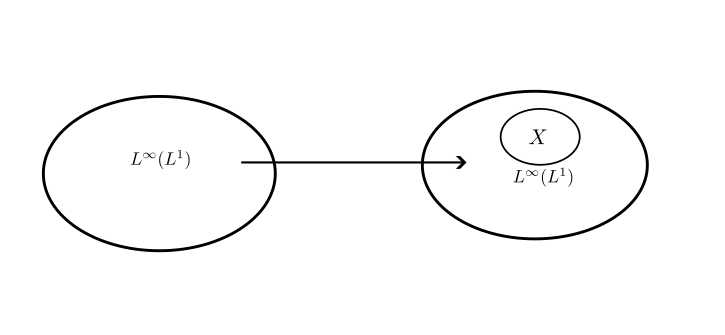
\includegraphics[scale=0.2]{figures/compactness.png}
 %  \end{figure}
 % \end{center}
    Let us check the that $M$ fulfills the conditions 1-3.
    For 1. note that for $v $ in a bounded subset of $L^{\infty}(L^{1} ) $
    \begin{align*}
      \|\nabla V \star  v\|_{L^{\infty} }\le C
    .\end{align*}
    Then by \autoref{aubin} $M(v,\sigma )$ is relatively compact in  $L^{2}(L^{2} ) $i.e $\exists  (v_j,\sigma_j)_{j \in  \mathbb{N}}$ s.t.
\begin{align*}
  \|M(v_j,\sigma_j) - u \|_{L^{2}(L^{2})} \xrightarrow{j \to \infty} 0 \quad \implies \quad  u_j \to  u \text{ a.e. }
.\end{align*}
we need to show 
\begin{align*}
  \|M(v_j,\sigma_j) - u\|_{L^{\infty}(L^{1} ) }  = \sup_t \int_{\mathbb{R}^{d} } \abs{u_j - u}(x) dx \xrightarrow{DCT}  0
.\end{align*}

    We check property 2. and note that if $\sigma=0$ our problem reduces to 
  \begin{align*}
  \begin{cases}
    &u_t - \Delta u + 0*\nabla*(\nabla V \star  u \ u) = v\\
    &u \rvert_{t=0} = 0*u_{0} 
  \end{cases}
  =  
  \begin{cases}
    &u_t - \Delta u  = v\\
    &u \rvert_{t=0} = 0  
  \end{cases}
 .\end{align*}
 which is just a Heat-Equation which when solved using the fundamental solution representation shows us that 
 \begin{align*}
  M(v,0) =  0 \quad \forall  v \in  L^{\infty}(L^{1} )
 .\end{align*}
 Property (3) is true since we chose $U = L^{\infty} $\\[1ex]
 This means we can apply \nameref{schauder_fixpoint}and get a fix point  $M(*,1)$ which is a solution  to 
 \begin{align*}
  \begin{cases}
    &u_t - \Delta u + \nabla*(\nabla V \star  u \ u) = 0 \quad  \\
    &\nabla V \in  L^{\infty}\\
    &u \rvert_{t=0} = u_{0}\ge 0  \quad \\
    &u_{0} \in L^{1}((1+\abs{x}^2)) \cap L^{2} 
  \end{cases}
 .\end{align*}
\end{proof}
\begin{theorem}[Uniqueness]
 If the nonlinear non-local \hyperref[pde_mve_apprach]{(PDE)} has a (weak) solution $u$ is unique.
\end{theorem}
\begin{proof}
 We suppose there are two (weak) solutions $u_{1},u_{2} \in  X$, then consider the difference 
 \begin{align*}
  w = u_{1} - u_{2}
 .\end{align*}
 which satisfies  (in a weak sense)
 \begin{align*}
  \begin{cases}
    &\partial_t w - \Delta w + \nabla *(\nabla V \star  u_{1} * w) + \nabla*(\nabla V \star w * u_{2}) = 0\\
    &w \rvert_{t=0} = 0
  \end{cases}
 .\end{align*}
take $w$ as a test function 
\begin{align*}
  \frac{1}{2} \frac{d}{dt} \int_{\mathbb{R}^{d} } w^2+ \int_{\mathbb{R}^{d} } \abs{\nabla w}^2 &\le \int_{\mathbb{R}^{d} } \abs{\nabla w *(\nabla V \star  u_{1})w}   + \int  \abs{\nabla w * (\nabla V \star  w)u_{2}} \\
                                                                                               &\le  \frac{1}{2} \int_{\mathbb{R}^{d} } \abs{\nabla w}^2 + C\int_{\mathbb{R}^{d} } (\abs{\nabla V \star  u_{1}}^2 \abs{w}^2 + \abs{\nabla V \star  w}^2 \abs{u_{2}}^2)\\
                                                                                               &\le  \|\nabla V \star  u_{1}\|_{L^{\infty}}^2 \int_{\mathbb{R}^{d} }  \abs{w}^2 + \|\nabla V \star  w\|_{L^\infty}^2 \|u_2\|_{L^{2} }^2\\
                                                                                               &\le C \int \abs{w}^2 %+ \|\nabla V\|_2^{2}\|w\|_2^{2}
.\end{align*}
where we used
\begin{align*}
  \essup_{x} \abs*{\int  \nabla V(x-y)w(y) dy}^2 \le \|\nabla V\|_2^{2}\|w\|_2^{2}  
.\end{align*}
then by Grönwalls inequality for $\forall  t \in  [0,\infty)$
\begin{align*}
  \frac{d}{dt} \int \abs{w}^2 \le C*\int \abs{w}^2 \implies \int_{\mathbb{R}^{d} }\abs{w(x,t)^2}dx \le  e^{Ct} \int_{\mathbb{R}^{d} } \abs{w(x,0)}^2 dx = 0
.\end{align*}
it follows $u_{1}=u_{2}$ a.e.
\end{proof}
\subsection{Back to the Makean-Vlasov Equation}
Let us see how all this ties back to the Makean-Vlasov Equation
\begin{align*}
  \text{(MVE)}\begin{cases}
    &dY(t) = (\nabla V \star  u)(Y(t)) dt + \sqrt{2}dW_t \\
    &Y(0)  = \xi \in  L^{2}(\Omega )\\
    &\mathcal{L}(\xi) = u_0 \in  L^{1}((1+\abs{x}^2)dx) \cap L^{2}(dx) \\
    &\mathcal{L}(Y) = u
  \end{cases}
.\end{align*}
Suppose now that $u$ is the solution of the  \hyperref[pde_mve_apprach]{(PDE)} obtained above, then consider 
for $\nabla V \in  \text{Lip}$ 
\begin{align*} 
  \text{(SDE)}\begin{cases}
    &dY(t) = (\nabla V \star  u)(Y(t)) dt + \sqrt{2}dW_t \\
    &Y(0)  = \xi \in  L^{2}(\Omega )\\
  \end{cases}
.\end{align*}
then the law of $\mathcal{L}(Y) = u$ satisfies 
then by convolution  $(\nabla V \star  u)$ is also Lipschitz, and by SDE theory there exists a unique solution $\exists! Y \in  \mathbb{L}^2([0,T])$  solving the (SDE).\\[1ex]
For $\forall  \phi  \in   C_0^{\infty}([0,T] \times  \mathbb{R}^{d} ) $, we have by It\^o's formula 
\begin{align*}
  \phi(Y(t),t) - \phi(Y(0),0) &= \int_0^{t}  \partial_t \phi(Y(s),s) + \nabla \phi(Y(s),s)* \nabla V \star u(Y(s),s) +\Delta \phi(Y(s),s) ds \\
                              &+ \int_0^{t}  \ldots  dW_s
.\end{align*}
Taking the expectation the stochastic term disappears, now suppose $\mu ^{Y} = \mathcal{L}(Y) $ then
\begin{align*}
  &\int_{\mathbb{R}^{d} } \phi(x,t) d\mu ^{Y}(x,t) - \int_{\mathbb{R}^{d} } \phi(x,0) u_0(x) dx \\
  &= \int_0^{t} \int_{\mathbb{R}^{d} } \partial_t \phi(x,s) + \nabla \phi(x,s) *(\nabla V \star u(x,s)) + \Delta  \phi(x,s) d\mu ^{Y}(x,s)ds 
.\end{align*}
Now to show that $\mu^Y = u$ which means that $\forall  \phi  \in  C_b$ 
\begin{align*}
  \int_{\mathbb{R}^{d} }\phi  d\mu ^{Y} = \int_{\mathbb{R}^{d} }  \phi  u dx
.\end{align*}
We show that the above PDE has a unique solution with $u_{0} \equiv 0$\\
We can rewrite the integral version in the weak sense as follows
\begin{align*}
  \partial_t \mu ^{Y} = \Delta \mu ^{Y}   - \nabla * (\nabla V \star  u * \mu ^{Y} )
.\end{align*}
\begin{remark}
There are two ways to prove $\mu^Y = 0$ \\
If $\phi  \in  \mathcal{C}_0^{\infty}([0,T)\times \mathbb{R}^{d} )$ and 
\begin{align*}
  &\int_{\mathbb{R}^{d} } \phi(x,T) d\mu ^{Y} - \underbrace{\int_{\mathbb{R}^{d} } \phi(x,0) d\mu^Y_0}_{=0}\\ \\
  &= \int_0^{T}\int_{\mathbb{R}^{d} }  (\partial_t \phi  + \Delta \phi  - \nabla \phi \nabla V \star u) d\mu^Y 
.\end{align*}
for $\forall  g \in  \mathcal{C}_0^{\infty}((0,T)\times \mathbb{R}^{d} ) $ we need to show 
\begin{align*}
  \int_0^{T} \int_{\mathbb{R}^{d}}   g(x,t) \mu^Y  = 0
.\end{align*}
the problem is reduced to  show that
\begin{align*}
  \begin{cases}
    &\partial_t \phi  + \Delta  \phi  - \nabla \phi  * \nabla V \star  u = g\\
    &\phi(x,T) = 0
  \end{cases}
.\end{align*}
solving this backwards PDE would go beyond the scope of this lecture and is just mentioned for completeness.\\[1ex]
\end{remark}
Instead we use a secondary method, for $\forall  \phi  \in  C_0^{\infty}([0,T)\times \mathbb{R}^{d} ) $
\begin{align*}
  \text{(\#)} &\int_{\mathbb{R}^{d} } \phi(x,t)  d\mu^Y(x) - \underbrace{\int_{\mathbb{R}^{d} } \phi(x,0) d\mu^Y_0}_{=0}\\
  &= \int_0^{t}\int_{\mathbb{R}^{d} }  (\partial_t \phi  + \Delta \phi  - \nabla \phi \nabla V \star u) d\mu^Y 
\end{align*}
then for fixed $\tilde{t} \in  (0,T)$ we want to show for $\forall  g \in  \mathcal{C}_0^{\infty}(\mathbb{R}^{d} ) $
\begin{align*}
  \int_{\mathbb{R}^{d} }g(x) d\mu^Y(x) = 0
.\end{align*}
now if we can find for any given $g$ the following problem 
\begin{align*}
  \begin{cases}
    &\partial_t \phi  + \Delta  \phi  - \nabla \phi *(\nabla V \star u) = 0\\
    &\phi(x,t) = g(x)
  \end{cases}
.\end{align*}
has a solution $\phi$, which can be viewed as a test function to be plugged into \# then 
\begin{align*}
  \mu ^{Y}  = 0 \text{ a.e. in }  \mathbb{R}^{d} 
.\end{align*}
The idea is now to suppose $\supp g \subset  B_{\frac{R}{2}}$, then we consider the corresponding problem 
\begin{align*}
  \begin{cases}
    &\partial_t w_{R,\epsilon} + \Delta w_{R,\epsilon} -\nabla w_{R,\epsilon} * j_{\epsilon} \star  (\nabla V \star  u) = 0\\
    &w_{R,\epsilon} \rvert_{\partial B_{R}} =  0\\
    &w_{R,\epsilon} \rvert_{t = \tilde{t} }  = g
  \end{cases}
.\end{align*}
how to solve this linear parabolic equation is part of the lecture PDE, here we just use the result i.e.
there exists a unique solution 
\begin{align*}
  w_{R,\epsilon} \in  C^{\infty}(\overline{B_R} \times  [0,\tilde{t} ] ) \text{ with } w_{R,\epsilon} \rvert_{\partial B_R} = 0
.\end{align*}
$w_{R,\epsilon}$ should be a candidate  for $\phi $, however it is not in $C_0^{\infty}(\mathbb{R}^{d} \times  [0,\tilde{t} ] ) $,
To overcome this difficulty we introduce a cutoff function  
\begin{align*}
  C_0^{\infty}(\mathbb{R}^{d} ) \ni \psi_{R} &=  \begin{cases}
      1 &\abs{x} \le \frac{R}{2}\\
      \text{smooth in between} & \\
      0 &\abs{x} \ge R
    \end{cases}\\
    \abs{\nabla \psi_R} &\le \frac{C}{R} \\
    \abs{\Delta  \psi_R} &\le \frac{C}{R}
.\end{align*}
we use $\psi_R * w_{R,\epsilon}$ as a test function, then it holds
\begin{align*}
  \psi_{R}*w_{R,\epsilon} \rvert_{t = \tilde{t} } = g
.\end{align*}
and 
\begin{align*}
  &\int_{\mathbb{R}^{d} } g(x)d\mu^{Y}(x,\tilde{t} ) - 0 = \int_0^{\tilde{t} } \int_{\mathbb{R}^{d} }  (\partial_t  + \Delta -  \nabla V \star  j_{\epsilon} \star u * \nabla)(w_{R,\epsilon} \psi_R) d\mu^Y(x,t)\\
.\end{align*}
using that $w_{R,\epsilon}$ is solution to the above equation 
\begin{align*}
  &\int_{0}^{\tilde{t} } \int_{\mathbb{R}^{d} } \underbrace{(\partial_t  + \Delta -  \nabla V \star j_{\epsilon} \star u * \nabla) w_{R,\epsilon}}_{=0}*\psi_{R} d\mu^Y \\
  &+  \int_0^{\tilde{t} } \int_{\mathbb{R}^{d} } (2 \nabla \psi_R * \nabla w_{R,\epsilon} + w_{R,\epsilon} \Delta \psi_{R} - \nabla V \star  u *w_{R,\epsilon}*\nabla \psi_{R}) d\mu^Y \\
  &+ \int_0^{\tilde{t} } \int_{\mathbb{R}^{d} }  (\nabla V \star  j_{\epsilon} \star  u - \nabla V \star  u) * \nabla w_{R,\epsilon}\psi_{R} d\mu^Y\\
  &= I + II + III
.\end{align*}
if we have that $\|\nabla w_{R,\epsilon}\|_{L^{\infty} } + \|w_{R,\epsilon}\|_{L^{\infty} } \le  C$ uniformly in $R$ and $\epsilon$ (Omit the proof),
then $II$ can be bounded as follows
\begin{align*}
  \abs{II}\le \|\mu^Y\|_{L^{\infty}(L^{1} ) } (\|\nabla w_{R,\epsilon}\|_{\infty}*\|\nabla \psi_R\|_{\infty}+\|w_{R,\epsilon}\|_{\infty}*\|\Delta  \psi_R\|_{\infty} +\|\nabla V \star  u\|_{\infty} * \|w_{R,\epsilon}\|\|\nabla \psi_R\|_{\infty})
.\end{align*}
For $III$ 
\begin{align*}
  \abs{III}&\le C*\|\nabla V \star  j_{\epsilon} \star u - \nabla V \star  u \|_{\infty} \\
           &= \abs*{\int j_{\epsilon}(x-y)(\nabla V \star  u (y) - \nabla V \star  u(x)) dy}\\
           &\le  \|D^2 V \star  u \|_{\infty} C \epsilon ^2 \\
           &\xrightarrow{} 0
.\end{align*}
% since $u$ as a solution of (PDE) it is also a solution of the (LDPE) 
% the proof $u = \mu ^{Y}$ can be reduced to show that (LPDE) has a unique measure valued solution.\\
% Let $\tilde{\mu } \in  L^{\infty}(L^{1} )  $ be a solution for $\forall \phi  \in  \mathcal{C}_0^{\infty}([0,T);\mathbb{R}^{d} ) $
% \begin{align*}
%   \int_0^{T} \int_{\mathbb{R}^{d} }  \tilde{u}  (\partial_t \phi  +  \Delta  \phi  - \nabla \phi  * \nabla V \star  u) dx dt = 0
% .\end{align*}
% then $\tilde{u} = 0 $ implies the uniqueness of (LPDE), which means we need to show for $\forall  g \in  \mathcal{C}_c^{\infty}(\mathbb{R}^{d} \times [0,T] )  $
% it holds 
% \begin{align*}
%   \int_0^{T}  \int_{\mathbb{R}^{d } } \tilde{u}  g dx dt = 0
% .\end{align*}
% if $\exists  \phi $ s.t. $g = \partial_t \phi  + \Delta  \phi  - \nabla \phi  * \nabla V \star  u$
